\section{Immunologische Grundlagen}
\textbf{Kushagr Sinha}

%Bei den autoimmunen Enzephalitiden kann man schon am Namen erkennen, dass es sich hier um eine autoimmune Krankheit handelt. Was eine autoimmune Krankheit ist, wie diese entsteht sowie die wichtigsten Grundlagen dazu, werden in diesem Kapitel erklärt.

Bei den autoimmunen Enzephalitiden handelt es sich um entzündliche Erkrankungen des Gehirns, bei denen das Immunsystem fehlgeleitet ist und dadurch körpereigene Stoffe angreift (= autoimmun). Um diese autoimmune Krankheit und ihre Entstehung zu verstehen, wird in diesem Kapitel zunächst auf die wichtigsten Grundlagen des gesunden und des fehlgeleiteten Immunsystems eingegangen.
\subsection{Prinzipien der Immunabwehr}

Das Immunsystem des menschlichen Körpers ist ebenso wie das Nervensystem äußerst komplex. Seine Hauptaufgabe besteht darin, den Körper vor Viren, Bakterien und anderen körperfremden Stoffen zu schützen.\footcite{Smith1999}\\

Außerdem wird das Immunsystem in zwei Systeme unterteilt:
\begin{itemize}
	\item das angeborene (unspezifische) Immunsystem
	\item das adaptive (spezifische) Immunsystem
\end{itemize}

Das angeborene Immunsystem wirkt im Falle eines Krankheitserregers als erstes, am schnellsten und unspezifisch, also ohne Erkennung spezifischer Antigene, indem es auf allgemein charakteristische Strukturen der Erreger reagiert.\footcite{MSDImmunsystem2026}

Das adaptive Immunsystem hingegen reagiert langsamer als das angeborene, wirkt aber spezifisch gegen die Antigene der Erreger. Außerdem bildet es ein immunologisches Gedächtnis, um beim Wiederauftreten des Pathogens dieses schneller und besser bekämpfen zu können. Die zwei wichtigsten Zellen dabei sind die T-Lymphozyten und die B-Lymphozyten.\footcite{MSDImmunsystem2026}

T-Lymphozyten übernehmen vorwiegend regulatorische und zellvermittelte Funktionen. T-Helferzellen koordinieren die Immunantwort, indem sie durch die Ausschüttung von Zytokinen die Aktivierung anderer Immunzellen steuern. Zytotoxische T-Zellen sind hingegen in der Lage, virusinfizierte oder entartete Körperzellen gezielt zu zerstören. Die präzise Zusammenarbeit dieser verschiedenen Zelltypen ermöglicht eine effektive und kontrollierte Immunabwehr.

%B-Lymphozyten spielen eine entscheidende Rolle bei der humoralen Immunantwort. Nach Aktivierung durch Antigenkontakt und Unterstützung durch T-Helferzellen differenzieren sie sich zu Plasmazellen, die große Mengen spezifischer Antikörper produzieren. Antikörper sind Proteine, die meist der Klasse der Immunglobuline G (IgG) angehören und eine charakteristische Y-förmige Struktur besitzen (siehe Abbildung \ref{fig:yfigure}). Die variablen Regionen an den Enden der Antikörper ermöglichen eine hochspezifische Bindung an Antigene. Durch diese Bindung können Krankheitserreger neutralisiert oder für andere Immunzellen markiert werden.\footcite{DocCheckLymphozyt, doccheck_igg}

B-Lymphozyten differenzieren sich nach Aktivierung durch Antigenkontakt und Unterstützung durch T-Helferzellen zu Plasmazellen, welche große Mengen spezifischer Antikörper produzieren. Antikörper sind Proteine, die meist der Klasse der Immunglobuline G (IgG) angehören und eine charakteristische Y-förmige Struktur besitzen (siehe Abbildung \ref{fig:yfigure}). Die variablen Regionen an den Enden der Antikörper ermöglichen eine hochspezifische Bindung an Antigene. Durch diese Bindung können Krankheitserreger neutralisiert oder für andere Immunzellen markiert werden.\footcite{DocCheckLymphozyt, doccheck_igg}


\begin{figure}[h] % [h] versucht, das Bild hier zu platzieren (hier), [t] für oben, [b] für unten
	\centering % Zentriert das Bild horizontal
	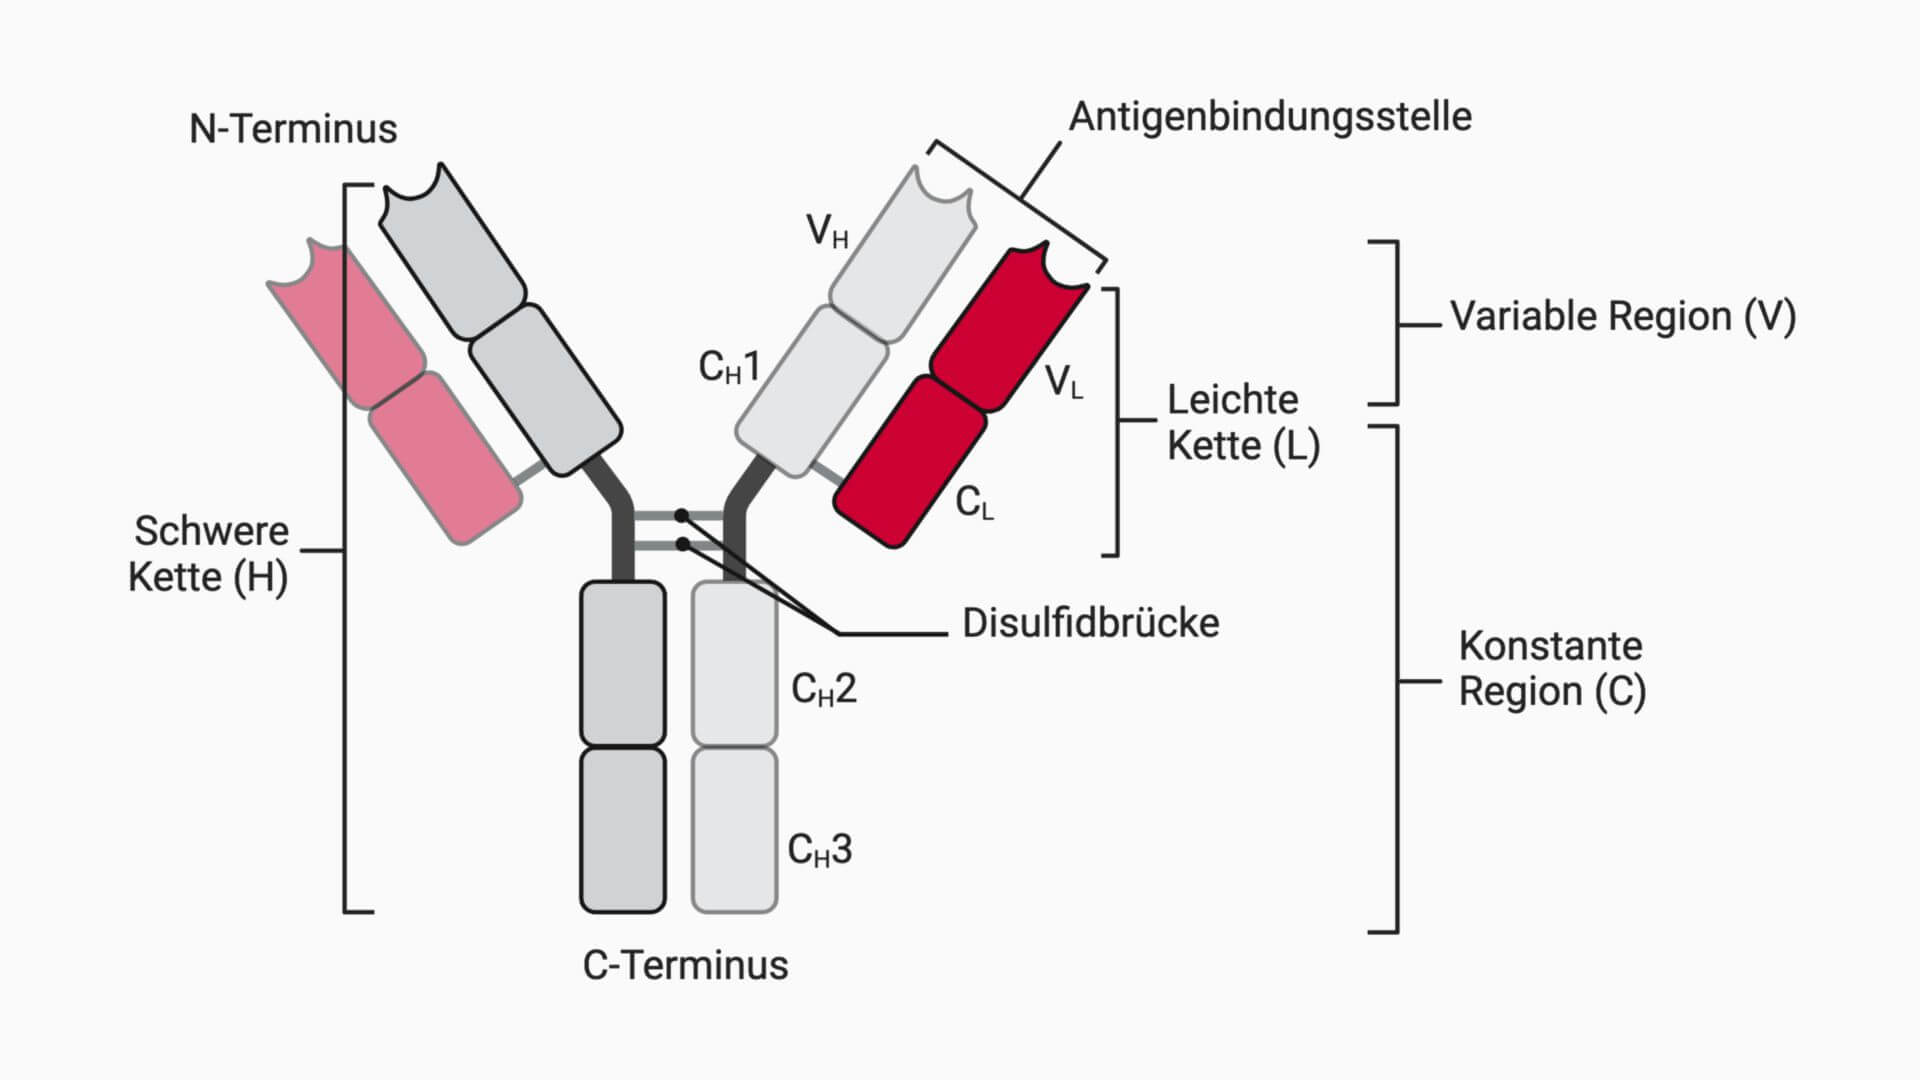
\includegraphics[width=0.91\textwidth]{abbildungen/IGGPI.jpg} % Lädt das Bild, skaliert es auf 80% der Textbreite
	\caption{Darstellung eines IgG-Antikörpers mit Beschriftung der strukturellen Regionen. \parencite{IGGbild_4u}} % Die Bildunterschrift
	\label{fig:yfigure} % Ein Label für Querverweise (z. B. "siehe Abbildung \ref{fig:beispielbild}")
\end{figure}

Damit beide Systeme miteinander kommunizieren können, gibt es dendritische Zellen. Diese gelten als Vermittler zwischen dem angeborenen und dem adaptiven Immunsystem. Sie erfüllen diese Aufgabe, indem sie Antigeninformationen von Erregern aufnehmen und diese dann an ihrer Oberfläche präsentieren. Dadurch werden Lymphozyten aktiviert, was wiederum zu einer spezifischen Immunantwort führt.\footcite{UniHeidelbergImmunologie2026}

Die Immunglobulinklasse G (IgG) umfasst vier Subklassen (IgG1 bis IgG4), die sich in ihrer Funktion unterscheiden und in Abbildung \ref{fig:yfigure} dargestellt sind. Während IgG1 und IgG3 oft Entzündungen durch das sogenannte Komplementsystem verstärken, nimmt IgG4 eine Sonderrolle ein: Es ist weniger entzündlich, neigt aber dazu, Bindungen zwischen Proteinen direkt zu blockieren.\footcite{doccheck_igg, AntwerpesIgG4}


\subsection{Mechanismen fehlgeleiteter Immunabwehr}

Ein zentrales Merkmal eines funktionierenden Immunsystems ist die Fähigkeit zur Selbsttoleranz. Das bedeutet, dass körpereigene Strukturen unter normalen Bedingungen nicht als Ziel einer Immunreaktion erkannt werden. Diese Eigenschaft ist entscheidend, um autoimmune Prozesse zu verhindern.\footcite{Smith1999}

Passiert bei der immunologischen Selbsttoleranz ein Fehler, greift das Immunsystem fälschlicherweise körpereigene Strukturen an. Dieser Vorgang wird als Autoimmunität bezeichnet. Erst wenn eine solche Reaktion zu messbaren Schäden an Organen oder Geweben führt und klinische Symptome aufweist, spricht man von einer Autoimmunerkrankung.\footcite{Fernandez2026}

%T- und B-Zellen entstehen beide im Knochenmark, durchlaufen jedoch bei ihrer Entwicklung spezifische Kontrollmechanismen, um eine Autoimmunität zu verhindern. Sie durchlaufen zunächst im Thymus bzw. im Knochenmark eine zentrale Toleranz, bei der geprüft wird, ob sie auf körpereigene Antigene reagieren. Ist dies der Fall, werden sie eliminiert.\footcite{DocCheckLymphozyt}

T- und B-Zellen reifen aus Vorläuferzellen im Thymus (daher auch T-Zelle) beziehungsweise im Knochenmark (B für engl. Bone Marrow). Bei ihrer Entwicklung durchlaufen sie eine zentrale Toleranz, bei der geprüft wird, ob sie auf körpereigene Antigene reagieren. Ist dies der Fall, werden sie eliminiert. Damit wird eine Autoimmunität verhindert.\footcite{DocCheckImmuntoleranz, DocCheckLymphozyt}

%Versagen die Toleranzmechanismen oder machen sie einen Fehler, sodass ein selbstreaktiver Lymphozyt überlebt und autoaggressive T-Zellen sowie Autoantikörper bildet, greift ein zusätzlicher Regulationsprozess ein, nämlich die periphere Toleranz. Hierbei unterdrücken regulatorische T-Zellen mithilfe von hemmenden Botenstoffen die Aktivierung solcher schädlicher Zellen oder lösen ihren Zelltod aus. Darüber hinaus kann die Zelle, wenn keine Entzündung vorliegt und somit keine kostimulatorischen Signale erhält, in einen Zustand der Inaktivität (Anergie) versetzt werden und somit keine Reaktion auslösen.\footcite{Macian2004, DocCheckImmuntoleranz}

Zusätzlich gibt es noch einen Selektionsprozess, die periphere Toleranz. Hierbei werden die T-Zellen gegen weitere Antigene getestet, die z. B. im Blut oder in Lymphknoten vorkommen. Dabei unterdrücken regulatorische T-Zellen mithilfe von hemmenden Botenstoffen die Aktivierung schädlicher Zellen oder lösen ihren Zelltod aus. Darüber hinaus kann die Zelle, wenn keine Entzündung vorliegt und sie somit keine kostimulatorischen Signale erhält, in einen Zustand der Inaktivität versetzt werden und somit keine Reaktion auslösen.\footcite{Macian2004, DocCheckImmuntoleranz}


%Zentral für die Entstehung der CASPR2-Enzephalitis ist ein Versagen der immunologischen Kontrollmechanismen: Selbstreaktive B-Zellen bilden Autoantikörper, die überwiegend zur IgG4-Subklasse gehören. Diese Antikörper gelangen über die Blut-Hirn-Schranke, eine normalerweise selektive Barriere zwischen Blutkreislauf und Gehirn, die das Eindringen schädlicher Stoffe verhindert, in das zentrale Nervensystem. Dort richten sie sich gegen das Protein CASPR2. Da IgG4-Antikörper kaum entzündliche Reaktionen auslösen, kommt es nicht zu einer direkten Zerstörung von Nervengewebe. Stattdessen beeinträchtigen sie die Funktion der Nervenzellen, indem sie die Stabilität von Kaliumkanälen stören. Die Folge ist eine erhöhte neuronale Erregbarkeit, die charakteristisch für die Erkrankung ist.\footcite{Patterson2018}

Die beschriebenen Mechanismen der immunologischen Selbsttoleranz sind auch für das Verständnis der Caspr2-Enzephalitis relevant. Bei dieser Erkrankung richtet sich die Immunantwort gegen körpereigene Strukturen des Nervensystems, insbesondere gegen das Protein Caspr2. (Im weiteren Verlauf wird daher betrachtet, welche Rolle Autoantikörper gegen Caspr2 bei der Erkrankung spielen.)
